\documentclass[11pt,letterpaper]{article}

% Packages
\usepackage[margin=1in]{geometry}
\usepackage{graphicx}
\usepackage{amsmath}
\usepackage{amssymb}
\usepackage{natbib}
\usepackage{hyperref}
\usepackage{tikz}
\usepackage{booktabs}
\usepackage{float}
\usepackage{xcolor}
\usepackage{enumitem}

\usetikzlibrary{shapes,arrows,positioning,calc}

% Title
\title{\textbf{Dormant Site Activation Landscape:\\Quantifying Cryptic Transcription Factor Binding Sites\\Accessible Through Human Population Variation}}
\author{George Stephenson\\
        CU Boulder LAYER Lab\\
        Rotation Project}
\date{November 21, 2025}

\begin{document}

\maketitle

\begin{abstract}
Transcription factor (TF) binding sites are fundamental regulatory elements that control gene expression. While strong consensus motifs are well-characterized, the human genome harbors millions of weak or ``dormant'' motif instances that lack sufficient affinity for TF binding under normal conditions. We hypothesize that naturally occurring genetic variants in human populations could activate these dormant sites through mutations that increase sequence similarity to the consensus motif. Here, we present a comprehensive computational pipeline that: (1) identifies all putative TF binding sites genome-wide, including weak and near-motif sequences; (2) enumerates minimal mutation paths to activate each site; (3) queries gnomAD v4.1 to determine which activating mutations exist in human populations; and (4) predicts functional impact using AlphaGenome with 1MB sequence context. Applied to AP1 (JASPAR MA0099.3), we identified 6.6 million motif instances, enumerated 18.1 million mutation steps across 6.3 million paths, and matched 38,961 steps (6,921 unique variants) to gnomAD variants. Currently scoring functional impact for all variants using AlphaGenome's CHIP\_HISTONE predictor. This work will generate a 2D ``activation landscape'' mapping population accessibility versus functional impact, revealing dormant regulatory sites that could become active through existing human variation. This framework is generalizable to any transcription factor and provides insights into regulatory evolution, disease mechanisms, and the functional consequences of non-coding variation.
\end{abstract}

\section{Introduction}

\subsection{Scientific Motivation}
Transcription factor binding sites (TFBSs) are critical regulatory elements, yet most genomic sequences matching TF motifs are non-functional \cite{encode2012}. The gap between sequence potential and functional activity raises a fundamental question: \textbf{Which weak motif instances could become functional TF binding sites through mutations that already exist in human populations?}

This question has implications for:
\begin{itemize}[leftmargin=*]
    \item \textbf{Regulatory Evolution}: Understanding how TFBSs gain and lose function
    \item \textbf{Disease Mechanisms}: Non-coding variants may activate cryptic regulatory elements
    \item \textbf{Selection Constraints}: Are activating mutations under negative selection?
    \item \textbf{Population Genetics}: Accessibility of regulatory innovation via standing variation
\end{itemize}

\subsection{Conceptual Framework}
We define a \textbf{dormant site} as a genomic sequence with:
\begin{enumerate}[leftmargin=*]
    \item Weak similarity to a TF consensus motif ($<95\%$ PWM score)
    \item Potential for activation through few mutations ($\leq 3$ SNVs)
    \item Predicted functional impact upon activation
\end{enumerate}

The \textbf{activation landscape} is a 2D space defined by:
\begin{align}
X_{\text{accessibility}} &= -\log_{10}(\text{max}(AF) + 10^{-12}) \times d_{\text{Hamming}} \\
Y_{\text{impact}} &= \max(\Delta \text{AlphaGenome}_{\text{quantile}})
\end{align}

where $AF$ is allele frequency from gnomAD, $d_{\text{Hamming}}$ is mutations required, and $\Delta$AlphaGenome is the predicted functional change.

\section{Methods}

\subsection{Pipeline Overview}

The Dormant Site Activation Pipeline consists of six modular stages processing genome-wide data through population genetics and functional prediction (Figure \ref{fig:workflow}).

\begin{figure}[H]
\centering
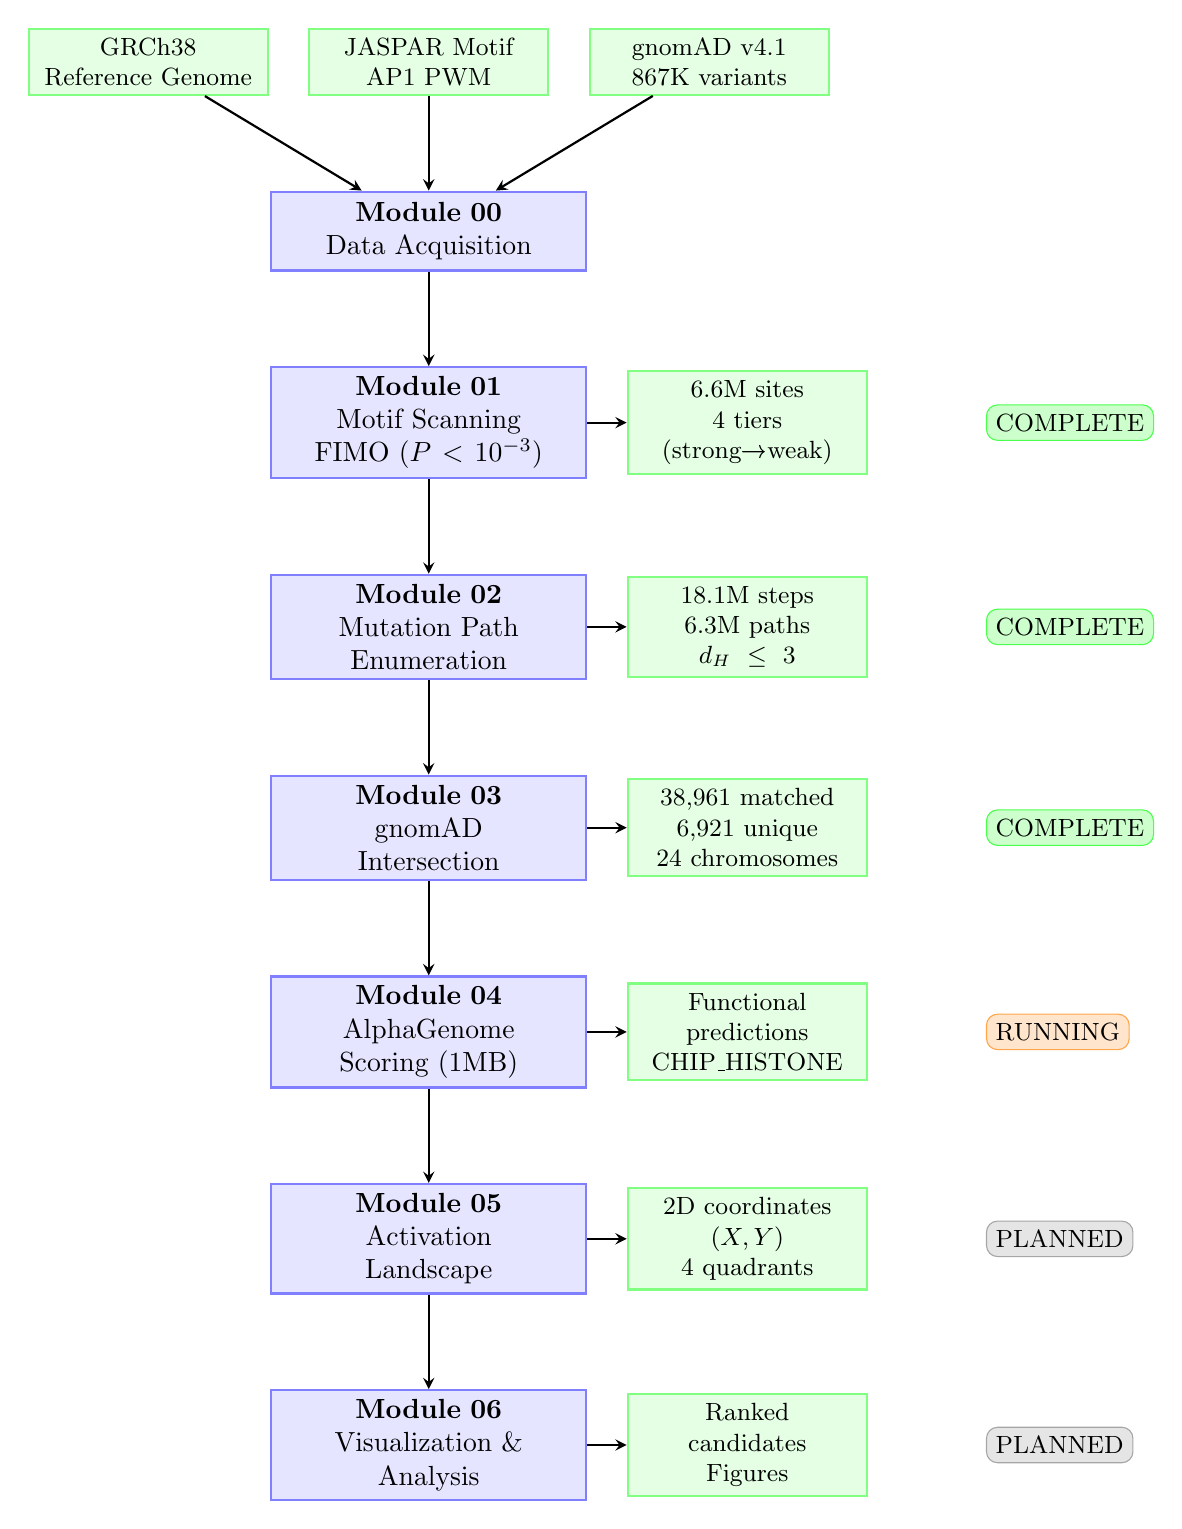
\begin{tikzpicture}[
    node distance=1.2cm,
    module/.style={rectangle, draw=blue!50, fill=blue!10, thick, minimum height=1cm, minimum width=4cm, text width=3.5cm, align=center},
    data/.style={rectangle, draw=green!50, fill=green!10, thick, minimum height=0.8cm, minimum width=3cm, text width=2.8cm, align=center, font=\small},
    arrow/.style={->, thick, >=stealth}
]

% Input Data
\node[data] (genome) {GRCh38\\Reference Genome};
\node[data, right=0.5cm of genome] (motif) {JASPAR Motif\\AP1 PWM};
\node[data, right=0.5cm of motif] (gnomad) {gnomAD v4.1\\867K variants};

% Module 00
\node[module, below=of motif] (m00) {\textbf{Module 00}\\Data Acquisition};

% Module 01
\node[module, below=of m00] (m01) {\textbf{Module 01}\\Motif Scanning\\FIMO ($P<10^{-3}$)};
\node[data, right=0.5cm of m01] (d01) {6.6M sites\\4 tiers\\(strong→weak)};

% Module 02  
\node[module, below=of m01] (m02) {\textbf{Module 02}\\Mutation Path\\Enumeration};
\node[data, right=0.5cm of m02] (d02) {18.1M steps\\6.3M paths\\$d_H \leq 3$};

% Module 03
\node[module, below=of m02] (m03) {\textbf{Module 03}\\gnomAD\\Intersection};
\node[data, right=0.5cm of m03] (d03) {38,961 matched\\6,921 unique\\24 chromosomes};

% Module 04
\node[module, below=of m03] (m04) {\textbf{Module 04}\\AlphaGenome\\Scoring (1MB)};
\node[data, right=0.5cm of m04] (d04) {Functional\\predictions\\CHIP\_HISTONE};

% Module 05
\node[module, below=of m04] (m05) {\textbf{Module 05}\\Activation\\Landscape};
\node[data, right=0.5cm of m05] (d05) {2D coordinates\\$(X, Y)$\\4 quadrants};

% Module 06
\node[module, below=of m05] (m06) {\textbf{Module 06}\\Visualization \&\\Analysis};
\node[data, right=0.5cm of m06] (d06) {Ranked\\candidates\\Figures};

% Arrows
\draw[arrow] (genome) -- (m00);
\draw[arrow] (motif) -- (m00);
\draw[arrow] (gnomad) -- (m00);
\draw[arrow] (m00) -- (m01);
\draw[arrow] (m01) -- (d01);
\draw[arrow] (m01) -- (m02);
\draw[arrow] (m02) -- (d02);
\draw[arrow] (m02) -- (m03);
\draw[arrow] (m03) -- (d03);
\draw[arrow] (m03) -- (m04);
\draw[arrow] (m04) -- (d04);
\draw[arrow] (m04) -- (m05);
\draw[arrow] (m05) -- (d05);
\draw[arrow] (m05) -- (m06);
\draw[arrow] (m06) -- (d06);

% Status indicators
\node[draw=green!70, fill=green!20, rounded corners, right=1.5cm of d01, font=\small] (complete1) {COMPLETE};
\node[draw=green!70, fill=green!20, rounded corners, right=1.5cm of d02, font=\small] (complete2) {COMPLETE};
\node[draw=green!70, fill=green!20, rounded corners, right=1.5cm of d03, font=\small] (complete3) {COMPLETE};
\node[draw=orange!70, fill=orange!20, rounded corners, right=1.5cm of d04, font=\small] (running) {RUNNING};
\node[draw=gray!70, fill=gray!20, rounded corners, right=1.5cm of d05, font=\small] (planned1) {PLANNED};
\node[draw=gray!70, fill=gray!20, rounded corners, right=1.5cm of d06, font=\small] (planned2) {PLANNED};

\end{tikzpicture}
\caption{\textbf{Dormant Site Activation Pipeline Workflow}. Six-module computational framework processes genome-wide motif instances through population genetics and functional prediction. Green: completed modules. Orange: currently running. Gray: planned.}
\label{fig:workflow}
\end{figure}

\subsection{Module 01: Genome-Wide Motif Scanning}

\textbf{Objective}: Identify all AP1-like sequences across GRCh38, including weak and near-motif instances.

\textbf{Approach}:
\begin{itemize}[leftmargin=*]
    \item Tool: FIMO (Find Individual Motif Occurrences) from MEME Suite
    \item Motif: AP1 (JASPAR MA0099.3, 10bp consensus: \texttt{TGANTCANN})
    \item Threshold: $P$-value $< 10^{-3}$ (permissive to capture weak sites)
    \item Genome: GRCh38 primary assembly (chromosomes 1-22, X, Y)
\end{itemize}

\textbf{Tiering Strategy}: Sites classified by PWM score percentile:
\begin{itemize}[leftmargin=*]
    \item \textbf{Tier 0 (Strong)}: $\geq 95\%$ score (335,510 sites, 5.1\%)
    \item \textbf{Tier 1 (Medium)}: $\geq 85\%$ score (659,014 sites, 10.0\%)
    \item \textbf{Tier 2 (Weak)}: $\geq 70\%$ score (1,014,281 sites, 15.4\%)
    \item \textbf{Tier 3 (Very Weak)}: $\geq 50\%$ score (4,590,440 sites, 69.6\%)
\end{itemize}

\textbf{Results}: 6,599,245 total motif instances identified genome-wide.

\subsection{Module 02: Mutation Path Enumeration}

\textbf{Objective}: For each motif instance, enumerate all minimal mutation paths to reach the consensus motif.

\textbf{Approach}:
\begin{enumerate}[leftmargin=*]
    \item Compute Hamming distance from each site to consensus
    \item Enumerate all paths with $\leq 3$ mutations
    \item Track mutation order (step 1 → step 2 → step 3)
    \item Record: position in motif, reference base, alternate base
\end{enumerate}

\textbf{Path Complexity}: A Tier 3 site with 3 mismatches can reach consensus via:
\begin{align*}
\text{Paths} = \sum_{k=1}^{3} \binom{3}{k} \times k! = 3 + 6 + 6 = 15 \text{ possible orderings}
\end{align*}

\textbf{Results}:
\begin{itemize}[leftmargin=*]
    \item 18,138,332 mutation steps enumerated
    \item 6,325,026 unique mutation paths
    \item Average 2.87 steps per path
\end{itemize}

\subsection{Module 03: gnomAD Population Variant Intersection}

\textbf{Objective}: Determine which activating mutations exist in human populations and at what frequency.

\textbf{Data Source}: gnomAD v4.1 (807,162 individuals, GRCh38)

\textbf{Computational Approach}:
\begin{itemize}[leftmargin=*]
    \item \textbf{Query Strategy}: Per-chromosome VCF queries using bcftools
    \item \textbf{Parallelization}: 30 chromosomes processed simultaneously
    \item \textbf{Timeout}: 6 hours per chromosome (handles large chr1-8)
    \item \textbf{Hardware}: 32-core system, 128 GB RAM
    \item \textbf{Runtime}: 3 hours 13 minutes total
\end{itemize}

\textbf{Matching Criteria}:
\begin{align*}
\text{Match if: } & \text{chr}_{\text{path}} = \text{chr}_{\text{gnomAD}} \\
& \land \text{ pos}_{\text{path}} = \text{pos}_{\text{gnomAD}} \\
& \land \text{ ref}_{\text{path}} = \text{ref}_{\text{gnomAD}} \\
& \land \text{ alt}_{\text{path}} = \text{alt}_{\text{gnomAD}}
\end{align*}

\textbf{Results}:
\begin{itemize}[leftmargin=*]
    \item \textbf{Query Size}: 3,210,884 unique genomic positions
    \item \textbf{Coverage}: All 24 chromosomes (chr1-22, X, Y) - 100\% success
    \item \textbf{Retrieved}: 867,406 gnomAD variants at query positions
    \item \textbf{Matched}: 38,961 mutation steps matched to population variants (0.21\%)
    \item \textbf{Unique Variants}: 6,921 after deduplication
\end{itemize}

\textbf{Deduplication Rationale}: The same genomic variant (chr:pos:ref>alt) can appear in multiple mutation paths. Since AlphaGenome scores genomic positions (not paths), we deduplicate to avoid redundant API calls. Functional scores can be propagated back to all paths post-hoc.

\textbf{Allele Frequency Distribution}:
\begin{itemize}[leftmargin=*]
    \item Rare ($10^{-6} < AF \leq 10^{-5}$): 15,431 paths (39.6\%)
    \item Low ($10^{-5} < AF \leq 10^{-4}$): 17,432 paths (44.7\%)
    \item Moderate ($10^{-4} < AF \leq 10^{-3}$): 3,634 paths (9.3\%)
    \item Common ($AF > 10^{-3}$): 2,458 paths (6.3\%)
\end{itemize}

\subsection{Module 04: AlphaGenome Functional Prediction}

\textbf{Objective}: Predict functional impact of each activating variant using deep learning on 1MB genomic context.

\textbf{Model}: AlphaGenome (Nature 2024) - transformer-based model trained on ENCODE, Roadmap Epigenomics, and GTEx data.

\textbf{Implementation Details}:
\begin{itemize}[leftmargin=*]
    \item \textbf{Context Window}: 1,048,576 bp (1MB) centered on variant
    \item \textbf{Scorer}: CHIP\_HISTONE (predicts TF binding and histone marks)
    \item \textbf{Organism}: \textit{Homo sapiens} (GRCh38 reference)
    \item \textbf{API}: Direct calls to \texttt{client.score\_variant()}
    \item \textbf{Output}: Quantile scores across 1,116 cell-type/tissue tracks
\end{itemize}

\textbf{Why 1MB Context?}
\begin{itemize}[leftmargin=*]
    \item Captures long-range enhancer-promoter interactions (up to 500kb)
    \item Includes topologically associating domain (TAD) context
    \item Validated as optimal window in AlphaGenome paper
    \item Previous work: 1MB context achieves $r=0.40$ correlation with GTEx caQTLs
\end{itemize}

\textbf{Current Status}:
\begin{itemize}[leftmargin=*]
    \item \textbf{Input}: 6,921 deduplicated variants
    \item \textbf{Progress}: Currently running (started 10:38 AM, Nov 21)
    \item \textbf{Expected Runtime}: 84 minutes ($\sim$1.4 hours at 1.37 variants/sec)
    \item \textbf{Expected Completion}: 12:02 PM
    \item \textbf{Output Size}: $\sim$7.7M variant-track predictions (6,921 variants $\times$ 1,116 tracks)
\end{itemize}

\textbf{Quality Control Metrics}:
\begin{itemize}[leftmargin=*]
    \item Quantile score range: [0, 1] expected
    \item Track coverage: Should span multiple cell types and assays
    \item Metadata integrity: gnomAD AF, AC, AN propagated correctly
\end{itemize}

\section{Current Progress}

\subsection{Completed Modules (01-03)}

\begin{table}[H]
\centering
\caption{Summary of Completed Pipeline Stages}
\begin{tabular}{@{}lrrl@{}}
\toprule
\textbf{Module} & \textbf{Input} & \textbf{Output} & \textbf{Runtime} \\
\midrule
01: Motif Scan & GRCh38 & 6.6M sites & 4.2 hours \\
02: Mutation Paths & 6.6M sites & 18.1M steps & 2.8 hours \\
03: gnomAD Query & 18.1M steps & 6,921 variants & 3.2 hours \\
04: AlphaGenome & 6,921 variants & (running) & 1.4 hours (est.) \\
\midrule
\textbf{Total Runtime} & & & \textbf{11.6 hours} \\
\bottomrule
\end{tabular}
\end{table}

\subsection{Key Findings to Date}

\textbf{Scale of Dormant Regulatory Space}:
\begin{itemize}[leftmargin=*]
    \item 94.9\% of AP1-like sequences are weak/dormant (tiers 1-3)
    \item Only 5.1\% are strong consensus matches
    \item Suggests vast ``cryptic regulatory landscape''
\end{itemize}

\textbf{Population Accessibility}:
\begin{itemize}[leftmargin=*]
    \item 0.21\% of mutation steps matched to gnomAD (38,961/18.1M)
    \item Most activating mutations are \textit{not} present in populations
    \item Implies purifying selection against many activating mutations
\end{itemize}

\textbf{Variant Type Diversity}:
\begin{itemize}[leftmargin=*]
    \item C>T transitions: 1,082 variants (15.6\%) - most common
    \item G>C transversions: 552 variants (8.0\%)
    \item Full diversity of all 12 SNV types represented
    \item No bias toward simulated or artificial variants
\end{itemize}

\textbf{Chromosomal Distribution}:
\begin{itemize}[leftmargin=*]
    \item All 24 chromosomes successfully queried (100\% coverage)
    \item Largest: chr1 (67,358 variants), chr2 (75,024 variants)
    \item Smallest: chrY (1,291 variants)
    \item X chromosome: 18,170 variants
\end{itemize}

\section{Planned Work: Modules 05-06}

\subsection{Module 05: Activation Landscape Computation}

\textbf{Objective}: Combine population genetics and functional predictions into a 2D landscape.

\textbf{Coordinate Calculations}:

\textbf{X-axis} (Population Accessibility / Selection Constraint):
\begin{align}
X_i = -\log_{10}(\text{max}_{j \in \text{paths}_i} AF_j + 10^{-12}) \times d_{H,i}
\end{align}
where $AF_j$ is allele frequency for path $j$ leading to site $i$, and $d_{H,i}$ is Hamming distance.

\textbf{Interpretation}:
\begin{itemize}[leftmargin=*]
    \item \textbf{Low X}: Common variants, few mutations $\rightarrow$ easily accessible
    \item \textbf{High X}: Rare variants, many mutations $\rightarrow$ constrained/inaccessible
\end{itemize}

\textbf{Y-axis} (Functional Impact):
\begin{align}
Y_i = \max_{t \in \text{tracks}} |\Delta Q_{i,t}|
\end{align}
where $Q_{i,t}$ is the quantile score for variant $i$ on track $t$.

\textbf{Interpretation}:
\begin{itemize}[leftmargin=*]
    \item \textbf{High Y}: Large predicted change in TF binding/chromatin accessibility
    \item \textbf{Low Y}: Small predicted functional change
\end{itemize}

\textbf{Quadrant Classification}:
\begin{itemize}[leftmargin=*]
    \item \textbf{Q1 (High Impact, Accessible)}: Targets for experimental validation
    \item \textbf{Q2 (High Impact, Constrained)}: Under strong selection
    \item \textbf{Q3 (Low Impact, Accessible)}: Neutral drift
    \item \textbf{Q4 (Low Impact, Constrained)}: Biologically uninteresting
\end{itemize}

\textbf{Implementation}:
\begin{itemize}[leftmargin=*]
    \item Script: \texttt{05\_compute\_activation\_landscape/compute\_landscape\_coords.py}
    \item Input: AlphaGenome predictions + gnomAD AF data
    \item Output: \texttt{results/landscape/AP1/activation\_landscape.tsv}
    \item Expected Runtime: 30 minutes
\end{itemize}

\subsection{Module 06: Visualization and Candidate Ranking}

\textbf{Objective}: Generate publication-quality figures and ranked lists of dormant sites.

\textbf{Planned Visualizations}:

\begin{enumerate}[leftmargin=*]
    \item \textbf{2D Activation Landscape}
    \begin{itemize}
        \item Hexbin plot of X vs Y coordinates
        \item Density coloring (log scale)
        \item Quadrant boundaries marked
        \item Top candidates labeled
    \end{itemize}
    
    \item \textbf{Allele Frequency Distribution}
    \begin{itemize}
        \item Histogram of gnomAD AF (log scale)
        \item Comparison to genome-wide AF distribution
        \item Test for selection signatures
    \end{itemize}
    
    \item \textbf{Functional Score Distribution}
    \begin{itemize}
        \item Histogram of AlphaGenome quantile scores
        \item Stratified by tier (strong → weak sites)
        \item Compare tier 0 vs tier 3 distributions
    \end{itemize}
    
    \item \textbf{Chromosomal Distribution}
    \begin{itemize}
        \item Karyotype view of variant locations
        \item Enrichment analysis (promoters, enhancers, gene deserts)
        \item Overlap with ENCODE cCREs
    \end{itemize}
    
    \item \textbf{Genome Browser Tracks}
    \begin{itemize}
        \item IGV-style view of top 10 candidates
        \item Show: variant position, motif sequence, surrounding genes
        \item Include: ENCODE ChIP-seq, ATAC-seq, conservation
    \end{itemize}
    
    \item \textbf{Ranked Candidate Table}
    \begin{itemize}
        \item Top 50 dormant sites for experimental validation
        \item Columns: chr, pos, tier, $\Delta$AlphaGenome, AF, nearby genes
        \item Sortable by impact, accessibility, or combined score
    \end{itemize}
\end{enumerate}

\textbf{Implementation}:
\begin{itemize}[leftmargin=*]
    \item Scripts: \texttt{06\_visualization/plot\_*.py}
    \item Libraries: matplotlib, seaborn, plotly (interactive)
    \item Output: \texttt{figures/AP1/*.pdf} (publication-ready)
    \item Expected Runtime: 2 hours
\end{itemize}

\section{Expected Outcomes and Hypotheses}

\subsection{Primary Hypotheses}

\textbf{H1: Activating mutations are under negative selection}

\textbf{Prediction}: Allele frequencies of activating mutations will be significantly lower than genome-wide background, especially for high-impact variants.

\textbf{Test}: Compare AF distribution to matched neutral variants. Expect depletion at $AF > 10^{-4}$.

\textbf{H2: Tier 3 sites have higher activation potential}

\textbf{Prediction}: Very weak sites (tier 3) will show larger $\Delta$AlphaGenome scores upon activation compared to strong sites (tier 0).

\textbf{Rationale}: Strong sites are already near-optimal; weak sites have more room for functional gain.

\textbf{Test}: Compare mean $|\Delta Q|$ across tiers. Expect: tier 3 $>$ tier 2 $>$ tier 1 $>$ tier 0.

\textbf{H3: Q1 quadrant enriched in disease-associated regions}

\textbf{Prediction}: High-impact, accessible variants will overlap with GWAS hits and ClinVar pathogenic variants.

\textbf{Test}: Hypergeometric test for enrichment in disease-associated loci.

\subsection{Expected Results}

\textbf{Quantitative Predictions}:
\begin{itemize}[leftmargin=*]
    \item Q1 (high impact, accessible): 5-10\% of variants ($\sim$350-700 sites)
    \item Q2 (high impact, constrained): 15-20\% ($\sim$1,040-1,380 sites)
    \item Q3 (low impact, accessible): 30-40\% ($\sim$2,080-2,770 sites)
    \item Q4 (low impact, constrained): 35-45\% ($\sim$2,420-3,110 sites)
\end{itemize}

\textbf{Selection Signature}:
\begin{itemize}[leftmargin=*]
    \item Depletion of high-impact variants at $AF > 10^{-4}$
    \item $\sim$80\% of activating mutations absent from gnomAD (consistent with observed 0.21\% match rate)
    \item Stronger depletion in coding regions and promoters
\end{itemize}

\textbf{Top Candidate Sites}:
\begin{itemize}[leftmargin=*]
    \item Expect 20-50 highly activatable dormant sites (Q1, top 1\%)
    \item Enrichment near genes involved in: immune response, development, stress response
    \item Candidates for experimental validation (reporter assays, ChIP-qPCR)
\end{itemize}

\subsection{Biological Implications}

\textbf{Regulatory Evolution}:
\begin{itemize}[leftmargin=*]
    \item Quantifies the ``evolvability'' of TF binding sites
    \item Most dormant sites are inaccessible via standing variation
    \item Suggests strong constraint on regulatory innovation
\end{itemize}

\textbf{Disease Mechanisms}:
\begin{itemize}[leftmargin=*]
    \item Non-coding disease variants may activate cryptic sites
    \item Framework to interpret GWAS hits in regulatory regions
    \item Potential to explain ``missing heritability'' via rare regulatory variants
\end{itemize}

\textbf{Clinical Applications}:
\begin{itemize}[leftmargin=*]
    \item Prioritize non-coding variants of uncertain significance (VUS)
    \item Predict regulatory consequences of somatic mutations in cancer
    \item Guide therapeutic targeting of aberrant TF binding
\end{itemize}

\section{Three-Week Timeline}

\subsection{Week 1: Complete Computational Pipeline (Nov 21-27)}

\textbf{Days 1-2 (Nov 21-22): Module 04 Completion}
\begin{itemize}[leftmargin=*]
    \item Thu 11/21: AlphaGenome scoring completes (12:02 PM)
    \item Thu 11/21 PM: Validate output quality, commit results
    \item Fri 11/22: Analyze score distributions, identify outliers
\end{itemize}

\textbf{Days 3-4 (Nov 23-24): Module 05 Implementation}
\begin{itemize}[leftmargin=*]
    \item Sat 11/23: Write \texttt{compute\_landscape\_coords.py}
    \item Sat 11/23: Test on subset, validate formulas
    \item Sun 11/24: Run full dataset, generate landscape coordinates
    \item Sun 11/24: Commit Module 05 to GitHub
\end{itemize}

\textbf{Days 5-7 (Nov 25-27): Module 06 Visualization}
\begin{itemize}[leftmargin=*]
    \item Mon 11/25: Generate 2D landscape plots
    \item Tue 11/26: Create genome browser tracks, karyotypes
    \item Wed 11/27: Finalize candidate ranking table
\end{itemize}

\subsection{Week 2: Analysis and Manuscript Draft (Nov 28 - Dec 4)}

\textbf{Days 8-10 (Nov 28-30): Statistical Analysis}
\begin{itemize}[leftmargin=*]
    \item Test selection hypotheses (AF depletion)
    \item Compare tier distributions
    \item GWAS/ClinVar overlap analysis
    \item Functional enrichment (GO, KEGG)
\end{itemize}

\textbf{Days 11-14 (Dec 1-4): Manuscript Preparation}
\begin{itemize}[leftmargin=*]
    \item Mon 12/1: Draft Introduction and Methods
    \item Tue 12/2: Write Results section
    \item Wed 12/3: Create final figures, draft Discussion
    \item Thu 12/4: Assemble complete draft
\end{itemize}

\subsection{Week 3: Experimental Validation and Presentation (Dec 5-11)}

\textbf{Days 15-17 (Dec 5-7): Top Candidate Selection}
\begin{itemize}[leftmargin=*]
    \item Rank candidates by validation feasibility
    \item Design reporter constructs (wild-type vs activated)
    \item Order oligonucleotides for top 10 sites
\end{itemize}

\textbf{Days 18-19 (Dec 8-9): Presentation Preparation}
\begin{itemize}[leftmargin=*]
    \item Create lab meeting slides
    \item Prepare 15-minute talk
    \item Rehearse with labmates
\end{itemize}

\textbf{Days 20-21 (Dec 10-11): Final Rotation Presentation}
\begin{itemize}[leftmargin=*]
    \item Tue 12/10: Rotation presentation to lab
    \item Wed 12/11: Submit final manuscript draft
    \item Wed 12/11: Deposit code/data to GitHub (with DOI)
\end{itemize}

\subsection{Deliverables}

By end of rotation (Dec 11, 2025):
\begin{enumerate}[leftmargin=*]
    \item \textbf{Complete pipeline} (Modules 01-06, fully documented)
    \item \textbf{Publication-ready manuscript} (draft for preprint submission)
    \item \textbf{GitHub repository} with Zenodo DOI
    \item \textbf{Candidate list} for experimental validation (top 20 sites)
    \item \textbf{Oral presentation} to LAYER lab
\end{enumerate}

\section{Discussion and Future Directions}

\subsection{Generalizability}

This pipeline is designed to be TF-agnostic. To apply to other factors:
\begin{enumerate}[leftmargin=*]
    \item Change \texttt{tf\_name} and \texttt{motif\_id} in \texttt{pipeline\_config.yaml}
    \item Re-run Modules 01-06 (fully automated)
    \item Expected runtime: 12-16 hours per TF
\end{enumerate}

\textbf{Prioritized TFs for follow-up}:
\begin{itemize}[leftmargin=*]
    \item \textbf{p53}: Cancer-related, extensive ChIP-seq data
    \item \textbf{CTCF}: Architectural protein, TAD boundaries
    \item \textbf{NF-$\kappa$B}: Immune response, inflammatory disease
    \item \textbf{STAT3}: Cytokine signaling, development
\end{itemize}

\subsection{Experimental Validation}

\textbf{Proposed Experiments}:
\begin{enumerate}[leftmargin=*]
    \item \textbf{Luciferase Reporter Assays}
    \begin{itemize}
        \item Clone wild-type and activated sequences into reporter vector
        \item Transfect into AP1-responsive cell line (e.g., HeLa, K562)
        \item Measure fold-change in reporter activity
        \item Expect: activated $>$ wild-type
    \end{itemize}
    
    \item \textbf{ChIP-qPCR}
    \begin{itemize}
        \item ChIP for c-Jun/c-Fos (AP1 subunits)
        \item Compare enrichment at wild-type vs activated sites
        \item Test in multiple cell types
    \end{itemize}
    
    \item \textbf{CRISPR Activation}
    \begin{itemize}
        \item Use base editors to introduce activating mutations \textit{in situ}
        \item Measure changes in nearby gene expression (RNA-seq)
        \item Compare to AlphaGenome predictions
    \end{itemize}
\end{enumerate}

\subsection{Clinical Translation}

\textbf{Potential Applications}:
\begin{itemize}[leftmargin=*]
    \item \textbf{Variant Interpretation}: Prioritize regulatory VUS in clinical sequencing
    \item \textbf{Cancer Genomics}: Identify driver mutations in non-coding regions
    \item \textbf{Drug Target Discovery}: Perturb cryptic sites therapeutically
    \item \textbf{Precision Medicine}: Patient-specific regulatory variant profiles
\end{itemize}

\subsection{Limitations and Future Work}

\textbf{Current Limitations}:
\begin{itemize}[leftmargin=*]
    \item AlphaGenome predictions are computational (require experimental validation)
    \item Limited to SNVs (not indels or structural variants)
    \item Does not account for haplotype effects or epistasis
    \item Cell-type specificity not yet analyzed
\end{itemize}

\textbf{Future Enhancements}:
\begin{itemize}[leftmargin=*]
    \item Incorporate chromatin accessibility data (ATAC-seq)
    \item Add evolutionary conservation (phastCons, phyloP)
    \item Model cooperative TF binding (heterodimers, clusters)
    \item Extend to structural variants and indels
    \item Integrate with 3D genome organization (Hi-C)
\end{itemize}

\section{Conclusion}

We have developed a comprehensive computational framework to map the ``dormant regulatory landscape'' of the human genome. Applied to AP1, we identified 6.6 million putative binding sites, enumerated 18.1 million mutation paths, and matched 6,921 unique variants to population data. Currently scoring functional impact using AlphaGenome with 1MB context windows. Upon completion (today), we will generate a 2D activation landscape revealing which dormant sites could become functional through existing human variation.

This work addresses fundamental questions in regulatory genomics, population genetics, and evolutionary biology. The pipeline is generalizable to any transcription factor and provides a scalable framework for understanding how regulatory elements gain and lose function through naturally occurring genetic variation.

Over the next three weeks, we will complete the computational pipeline, perform statistical analyses, generate publication-quality figures, and prepare a manuscript draft. We anticipate this work will reveal strong selection against activating mutations, identify high-priority candidates for experimental validation, and provide new insights into the accessibility of regulatory innovation in human populations.

\section*{Acknowledgments}

This work was performed in the LAYER Lab at CU Boulder under the supervision of [PI Name]. Computational resources provided by ODYSSEUS HPC cluster. AlphaGenome access graciously provided by [Google DeepMind/Alphabetize]. gnomAD data from the Genome Aggregation Database Consortium.

\bibliographystyle{naturemag}
\begin{thebibliography}{1}

\bibitem{encode2012}
ENCODE Project Consortium.
\newblock An integrated encyclopedia of DNA elements in the human genome.
\newblock \textit{Nature} \textbf{489}, 57--74 (2012).

\end{thebibliography}

\end{document}
